% ============================================================
%  ML IoT Lab – Presentation Template
%  HCMUT EE Machine Learning & IoT Lab
%  Faculty of Electrical & Electronics Engineering, HCMUT
% ============================================================

\documentclass[aspectratio=169, 10pt]{beamer}

% ---- Compiler-Independent Vietnamese support ----
\usepackage{ifxetex,ifluatex}
\newif\ifxetexorluatex
\ifxetex
  \xetexorluatextrue
\else
  \ifluatex
    \xetexorluatextrue
  \fi
\fi

\ifxetexorluatex
  \usepackage{fontspec}
\else
  \usepackage[utf8]{inputenc}
  \usepackage[T5]{fontenc}
  \usepackage{lmodern}
\fi
\usepackage[vietnamese, english]{babel}

\usefonttheme{serif}
\usepackage{beamerthemeMLIOT}   % custom theme (in same folder)

% ---- Additional packages ----
\usepackage{amsmath, amssymb}
\usepackage{booktabs}
\usepackage{multicol}
\usepackage{caption}
\usepackage{hyperref}
\usepackage[loadonly]{enumitem}
\usepackage{array}
\usepackage{pifont}
\usepackage{ragged2e}
\usepackage{siunitx}
\DeclareSIUnit\bps{bps}

% ---- Hyperlink colours ----
\hypersetup{
  colorlinks = true,
  urlcolor   = MLIOTaccent,
  linkcolor  = MLIOTblue,
  citecolor  = MLIOTblue
}

% ============================================================
%  PAPER METADATA
% ============================================================
\title{Hệ thống Điều khiển Xe Robot không dây sử dụng Cảm biến MPU6050 và PWM trên Vi điều khiển STM32F103}

\author[Nhóm 2]{\footnotesize Nguyễn Công Tú, Phạm Đỗ Hồng Phúc, Mạch Viễn An, Nguyễn Phúc Khải}

\setAffiliations{%
  Nhóm: PỎSCHE WITH NO BRAKES \\
  Mentor: Võ Quang Vinh%
}

\setCorrespondingAuthor{%
  *Email liên hệ: \href{mailto:an.machvien@hcmut.edu.vn}{an.machvien@hcmut.edu.vn}%
}

\setPaperID{Embedded-C-Group2}

\institute{%
  Machine Learning \& IoT Lab,
  Trường Đại học Bách Khoa - ĐHQG TP.HCM (HCMUT)%
}

\date{Tháng 8 / 2026}

% ============================================================
\begin{document}
\selectlanguage{vietnamese}
% ============================================================

% ------------------------------------------------------------
%  SLIDE 1 – Title Slide
% ------------------------------------------------------------
\begin{frame}[plain]
  \titlepage
\end{frame}

% ------------------------------------------------------------
%  SLIDE 2 – Outline
% ------------------------------------------------------------
\begin{frame}{Nội dung báo cáo}
  \begin{columns}[T]
    \begin{column}{0.6\textwidth}
      \setbeamerfont{enumerate item}{size=\large}
      \begin{enumerate}
        \setlength{\itemsep}{0.6em}
        \item {\large Giới thiệu đề tài \& Mục tiêu} 
        \item {\large Kiến trúc hệ thống tổng thể} 
        \item {\large Thuật toán điều khiển \& Triển khai phần cứng} 
        \item {\large Thực nghiệm \& Đánh giá kết quả} 
        \item {\large Demo thực tế \& Nhận xét} 
        \item {\large Kết luận \& Hướng phát triển} 
      \end{enumerate}
    \end{column}
    
    \begin{column}{0.38\textwidth}
      \begin{block}{Thông tin nhóm}
        \footnotesize
        \textbf{\textcolor{MLIOTnavy}{Nhóm:}}\\
        PỎSCHE WITH NO BRAKES\\
        \textbf{\textcolor{MLIOTnavy}{Lab:}}\\
        Machine Learning \& IoT Lab\\[0.3em]
        \textbf{\textcolor{MLIOTnavy}{Mentor:}}\\
        Võ Quang Vinh
      \end{block}
    \end{column}
  \end{columns}
\end{frame}

% ------------------------------------------------------------
%  SECTION 1: GIỚI THIỆU ĐỀ TÀI
% ------------------------------------------------------------
\begin{frame}{1. Giới thiệu — Đặt vấn đề \& Mục tiêu}
  \begin{columns}[T]
    % Cột 1
    \begin{column}{0.48\textwidth}
      \begin{block}{Đặt vấn đề \& Động lực}
        \begin{itemize}
          \item Các phương pháp điều khiển robot truyền thống (nút bấm, joystick) thiếu tính trực quan và kém tự nhiên.
          \item Cảm biến quán tính MEMS IMU (\textbf{MPU6050}) mở ra khả năng điều khiển thông minh dựa trên góc nghiêng bàn tay.
          \item Vi điều khiển \textbf{STM32F103} với nhân ARM Cortex-M3 cung cấp khả năng xử lý thời gian thực mạnh mẽ, giá thành rẻ.
        \end{itemize}
      \end{block}
    \end{column}
    % Cột 2
    \begin{column}{0.48\textwidth}
      \begin{block}{Mục tiêu đề tài}
        \begin{itemize}
          \item Thiết kế mạch cầm tay thu thập tư thế chuyển động nghiêng của tay.
          \item Truyền thông tin điều khiển không dây bằng Bluetooth \textbf{HC-05}.
          \item Xe nhận tín hiệu, giải mã và điều tốc động cơ bằng phương pháp băm xung \textbf{PWM} kết hợp lái vi sai.
          \item Tích hợp bộ lọc \textbf{Kalman} chống nhiễu và cơ chế dừng an toàn (\textbf{Fail-safe}).
        \end{itemize}
      \end{block}
    \end{column}
  \end{columns}
\end{frame}

% ------------------------------------------------------------
%  SECTION 2: KIẾN TRÚC HỆ THỐNG
% ------------------------------------------------------------
\begin{frame}{2. Kiến trúc hệ thống — Sơ đồ khối tổng thể}
  \begin{center}
    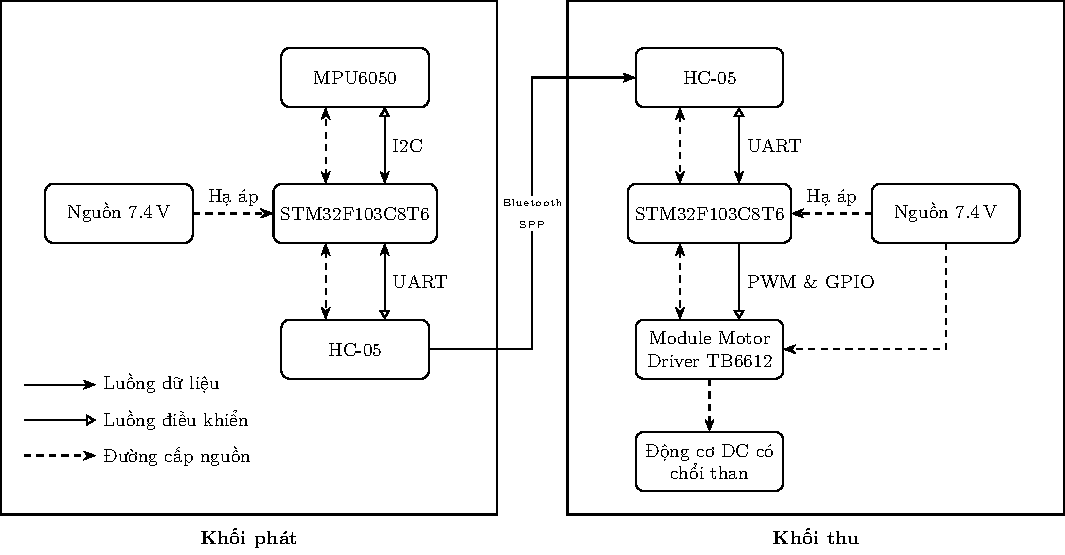
\includegraphics[height=0.68\textheight, keepaspectratio]{../Report/tikz/architecture.pdf}
  \end{center}
\end{frame}

\begin{frame}{2. Kiến trúc hệ thống — Luồng xử lý dữ liệu}
  \begin{columns}[T]
    \begin{column}{0.45\textwidth}
      \begin{block}{Các bước xử lý tuần tự}
        \begin{enumerate}
          \item \textbf{Thu thập dữ liệu:} STM32 đọc gia tốc ($A$) và vận tốc góc ($\omega$) từ MPU6050 qua I2C.
          \item \textbf{Ước lượng góc:} Lọc nhiễu góc nghiêng Pitch/Roll bằng thuật toán Kalman Filter.
          \item \textbf{Lập lệnh:} Ánh xạ góc nghiêng phi tuyến sang lệnh tốc độ (Deadzone \qty{\pm 8}{\degree}, Max \qty{\pm 60}{\degree}).
          \item \textbf{Truyền dữ liệu:} Gửi gói tin nối tiếp qua HC-05 (UART \qty{9600}{\bps}).
          \item \textbf{Thiết bị chấp hành:} Xe thu nhận tín hiệu $\to$ giải mã $	o$ băm xung PWM điều khiển động cơ.
        \end{enumerate}
      \end{block}
    \end{column}
    \begin{column}{0.52\textwidth}
      \begin{center}
        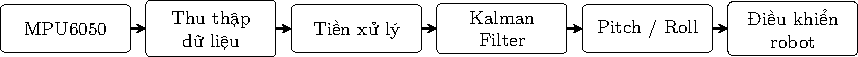
\includegraphics[width=\textwidth, height=0.68\textheight, keepaspectratio]{../Report/tikz/processing_flow.pdf}
      \end{center}
    \end{column}
  \end{columns}
\end{frame}

% ------------------------------------------------------------
%  SECTION 3: THUẬT TOÁN & TRIỂN KHAI
% ------------------------------------------------------------
\begin{frame}{3. Triển khai — Hardware \& Software Stack}
  \begin{columns}[T]
    \begin{column}{0.48\textwidth}
      \begin{block}{Cấu hình Phần cứng (Hardware)}
        \begin{itemize}
          \item \textbf{Vi điều khiển:} STM32F103C8T6 ở cả khối phát (tay cầm) và khối thu (xe).
          \item \textbf{Cảm biến:} MPU6050 (giao tiếp I2C1, chân PB6/PB7).
          \item \textbf{Bluetooth:} HC-05 (giao tiếp USART1, chế độ Master-Slave tự ghép nối).
          \item \textbf{Động cơ:} 2 mạch cầu H TB6612FNG lái độc lập 4 động cơ DC chổi than.
          \item \textbf{Nguồn:} Pin Li-ion \qty{3.7}{\volt} ở tay cầm; Pack pin \qty{7.4}{\volt} ở xe (hạ áp qua LM2596 và AMS1117).
        \end{itemize}
      \end{block}
    \end{column}
    
    \begin{column}{0.48\textwidth}
      \begin{block}{Cấu hình Phần mềm (Software)}
        \begin{itemize}
          \item Trình biên dịch C trên nền STM32 HAL.
          \item \textbf{Giao tiếp ngoại vi:}
            \begin{itemize}
              \item I2C: Tốc độ \qty{100}{\kilo\hertz}.
              \item UART: Baudrate \qty{9600}{\bps}, 8-N-1.
              \item \textbf{PWM: Tần số \qty{10}{\kilo\hertz}} trên Timer 2 (êm ái, giảm tiếng rít từ động cơ).
            \end{itemize}
          \item \textbf{Giải thuật chính:}
            \begin{itemize}
              \item Bộ lọc Kalman ước lượng góc Pitch/Roll.
              \item Điều khiển vi sai phi tuyến.
              \item Fail-safe ngắt động cơ khi mất sóng quá \textbf{\qty{300}{\ms}}.
            \end{itemize}
        \end{itemize}
      \end{block}
    \end{column}
  \end{columns}
\end{frame}

\begin{frame}{3. Triển khai — Sơ đồ nguyên lý Khối phát}
  \begin{columns}[T]
    \begin{column}{0.65\textwidth}
      \begin{center}
        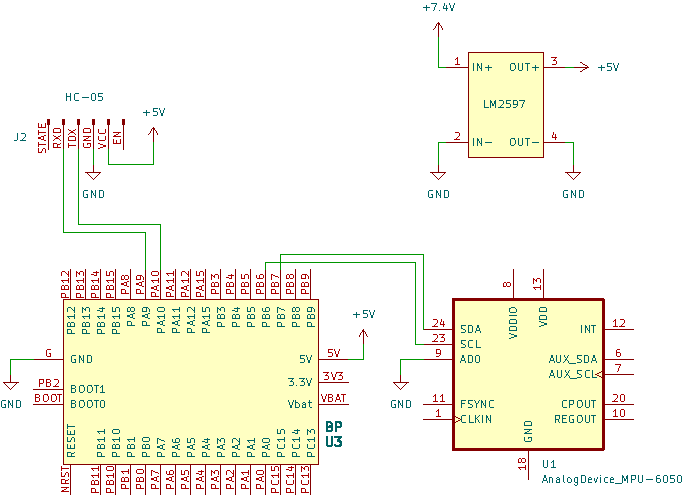
\includegraphics[width=\textwidth, height=0.68\textheight, keepaspectratio]{../Report/Schematic/Schematic-Transmitter.pdf}
      \end{center}
    \end{column}
    \begin{column}{0.31\textwidth}
      \begin{block}{Chi tiết kết nối}
        \footnotesize
        \begin{itemize}
          \item \textbf{Vi xử lý:} STM32F103C8T6 làm trung tâm điều khiển.
          \item \textbf{Cảm biến:} MPU6050 kết nối qua giao tiếp I2C1 (chân PB6/SCL, PB7/SDA).
          \item \textbf{Truyền thông:} HC-05 Master kết nối qua USART1 (PA9/TX, PA10/RX).
          \item \textbf{Nguồn cấp:} Pin Li-ion \qty{3.7}{\volt} kết hợp mạch hạ áp AMS1117-\qty{3.3}{\volt} cấp nguồn ổn định.
        \end{itemize}
      \end{block}
    \end{column}
  \end{columns}
\end{frame}

\begin{frame}{3. Triển khai — Sơ đồ nguyên lý Khối thu}
  \begin{columns}[T]
    \begin{column}{0.65\textwidth}
      \begin{center}
        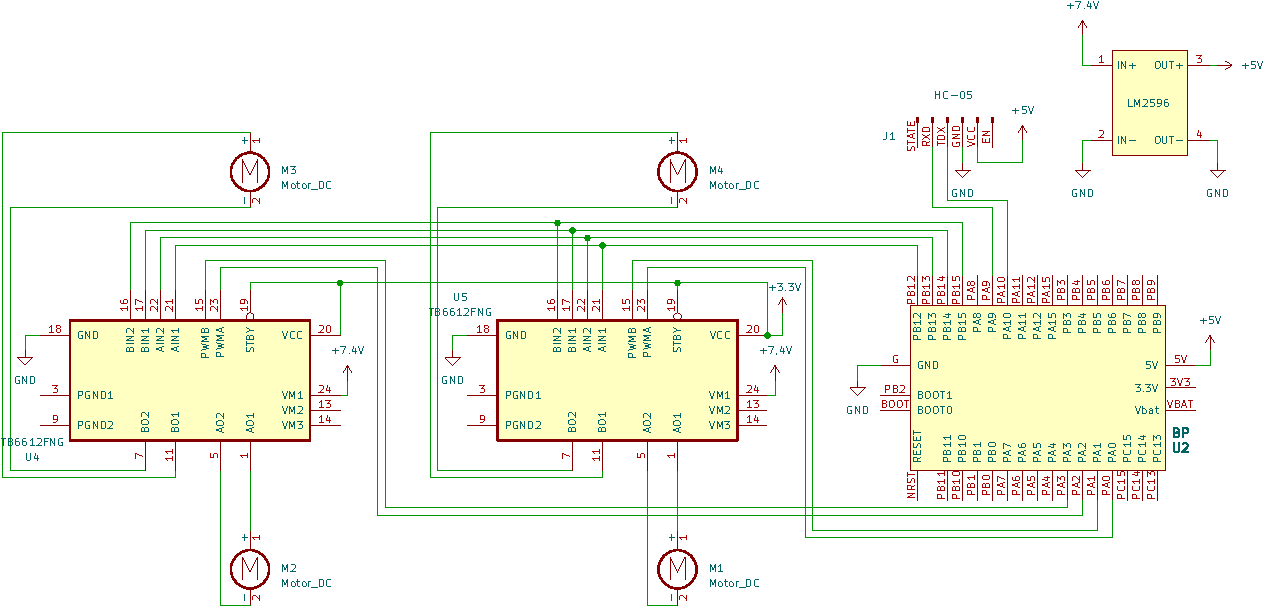
\includegraphics[width=\textwidth, height=0.68\textheight, keepaspectratio]{../Report/Schematic/Schematic-Receiver.pdf}
      \end{center}
    \end{column}
    \begin{column}{0.31\textwidth}
      \begin{block}{Chi tiết kết nối}
        \footnotesize
        \begin{itemize}
          \item \textbf{Vi xử lý:} STM32F103C8T6 nhận và giải mã gói tin điều khiển.
          \item \textbf{Bluetooth:} Module HC-05 Slave nhận dữ liệu qua USART1 (PA9/TX, PA10/RX).
          \item \textbf{Động lực:} 2 driver cầu H cầu TB6612FNG lái độc lập 4 bánh xe DC.
          \item \textbf{Nguồn cấp:} Pin Li-ion \qty{7.4}{\volt}, hạ áp qua mạch Buck LM2596 và LDO AMS1117-\qty{3.3}{\volt}.
        \end{itemize}
      \end{block}
    \end{column}
  \end{columns}
\end{frame}

\begin{frame}{3. Triển khai — Thuật toán lọc Kalman}
  \begin{columns}[T]
    \begin{column}{0.55\textwidth}
      \begin{block}{Tại sao sử dụng Kalman?}
        \footnotesize
        \begin{itemize}
          \item \textbf{Gia tốc kế (Accelerometer):} Tham chiếu góc dài hạn nhưng nhạy với rung và gia tốc động (nhiễu cao tần).
          \item \textbf{Con quay hồi chuyển (Gyroscope):} Phản ứng nhanh nhưng có bias và tích lũy trôi góc (drift) theo thời gian.
          \item \textbf{Bộ lọc Kalman (Kalman Filter):} Thực hiện dung hợp cảm biến (sensor fusion) thay vì lấy trung bình đơn giản.
        \end{itemize}
      \end{block}
      \vspace{0.4em}
      \begin{block}{Nguyên lý xử lý}
        \scriptsize
        \centering
        Gyroscope $\rightarrow$ Prediction \quad | \quad Accelerometer $\rightarrow$ Measurement Update \\
        $\Downarrow$ \\
        Estimated Angle (Góc ước lượng tối ưu)
      \end{block}
    \end{column}
    \begin{column}{0.41\textwidth}
      \begin{center}
        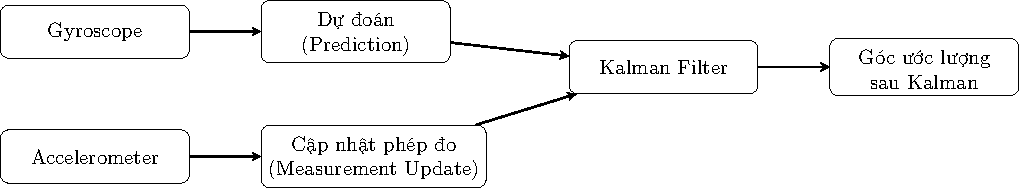
\includegraphics[width=\textwidth, height=0.68\textheight, keepaspectratio]{../Report/tikz/kalman_principle.pdf}
      \end{center}
    \end{column}
  \end{columns}
\end{frame}

\begin{frame}{3. Triển khai — Công thức bộ lọc Kalman}
  \begin{columns}[T]
    \begin{column}{0.48\textwidth}
      \begin{block}{Giải pháp \& Phương trình bộ lọc}
        \small
        \begin{itemize}
          \item \textbf{Trạng thái:}
            $$x_k = [\theta_k \quad b_k]^T$$
            \scriptsize (góc và bias con quay hồi chuyển)
          \item \small \textbf{Bước dự đoán (Prediction):}
            $$\theta_k^{-} = \theta_{k-1} + (\omega_{\text{measured}} - b_{k-1})\Delta t$$
            $$b_k^{-} = b_{k-1}$$
        \end{itemize}
      \end{block}
    \end{column}
    \begin{column}{0.48\textwidth}
      \begin{block}{Bước cập nhật (Measurement Update)}
        \small
        \begin{itemize}
          \item \textbf{Sai số đo lường (Innovation):}
            $$y_k = z_k - \theta_k^{-}$$
            \scriptsize (với $z_k = \theta_{\text{acc}}$ từ accelerometer)
          \item \small \textbf{Cập nhật trạng thái góc:}
            $$\theta_k = \theta_k^{-} + K_0 \cdot y_k$$
          \item \small \textbf{Cập nhật bias gyro:}
            $$b_k = b_{k-1} + K_1 \cdot y_k$$
        \end{itemize}
      \end{block}
    \end{column}
  \end{columns}
  \vspace{0.2em}
  \centering \scriptsize \textbf{Tham số trong code:} $Q_{\text{angle}} = 0.001$, $Q_{\text{bias}} = 0.003$, $R_{\text{measure}} = 0.03$.
\end{frame}

\begin{frame}{3. Triển khai — Hiệu chuẩn \& Chu kỳ xử lý}
  \begin{block}{Giải thuật Hiệu chuẩn (Calibration)}
    \small
    \begin{itemize}
      \item Khởi động hệ thống yêu cầu giữ thiết bị cầm tay nằm ngang cố định.
      \item Vi điều khiển thu thập \textbf{\num{200} mẫu} dữ liệu liên tiếp trong thời gian khởi chạy.
      \item Tính toán sai lệch tĩnh trung bình (bias) của Gyroscope và góc offset ban đầu.
      \item Triệt tiêu sai lệch này trong suốt quá trình chạy để thiết lập góc ban đầu $\approx \qty{0}{\degree}$.
    \end{itemize}
  \end{block}
  \begin{block}{Chu kỳ xử lý và Tần số thực thi}
    \small
    \begin{itemize}
      \item MPU6050 được cấu hình tần số lấy mẫu phần cứng ở mức \qty{100}{\hertz}.
      \item Vòng lặp chính khối phát chạy chu kỳ \textbf{\qty{10}{\ms}} ($f_{\text{loop}} = \qty{100}{\hertz}$) nhờ hàm \texttt{HAL\_Delay(10)}.
      \item Chu kỳ thực tế giữa hai lần đọc $\Delta t$ được tính toán động tại mỗi bước xử lý để đưa vào bộ lọc Kalman, tăng độ chính xác trong thời gian thực.
    \end{itemize}
  \end{block}
\end{frame}

\begin{frame}{3. Triển khai — Ánh xạ góc điều khiển \& Lái vi sai}
  \begin{columns}[T]
    % Cột 1
    \begin{column}{0.48\textwidth}
      \begin{block}{Ánh xạ phi tuyến (Expo Response)}
        \small
        \begin{itemize}
          \item Thiết lập vùng chết (\textbf{Deadzone}) \qty{\pm 8}{\degree} để loại bỏ rung tay nhẹ khi đứng yên.
          \item Thang đo góc hoạt động từ \qty{\pm 8}{\degree} đến \qty{\pm 60}{\degree} được ánh xạ phi tuyến sang giá trị điều khiển lái $u$ từ \num{0} đến \num{\pm 80}:
          $$u = \mathrm{sign}(\theta) \times \left( \frac{|\theta| - \num{8}}{\num{60} - \num{8}} \right)^2 \times \num{80}$$
          \item Giúp robot phản ứng mượt mà ở góc nghiêng nhỏ và nhạy ở góc nghiêng lớn.
        \end{itemize}
      \end{block}
    \end{column}
    % Cột 2
    \begin{column}{0.48\textwidth}
      \begin{block}{Lái vi sai động cơ (Differential Steering)}
        \small
        \begin{itemize}
          \item Chuỗi ký tự điều khiển \texttt{"F:\%d T:\%d\textbackslash n"} được truyền qua Bluetooth.
          \item Khối thu nhận $F$ (Forward) và $T$ (Turn) từ bộ phát (trong dải \num{\pm 80}), phối trộn tốc độ động cơ:
          \begin{align}
            V_{\text{left}} = \text{clamp}(F + T, \num{-100}, \num{100}) \notag \\
            V_{\text{right}} = \text{clamp}(F - T, \num{-100}, \num{100}) \notag
          \end{align}
          \item Hướng quay động cơ được điều khiển bằng GPIO (logic HIGH/LOW) và tốc độ bằng độ rộng xung PWM.
        \end{itemize}
      \end{block}
    \end{column}
  \end{columns}
\end{frame}

\begin{frame}{3. Triển khai — Lưu đồ giải thuật Khối phát}
  \begin{columns}[T]
    \begin{column}{0.65\textwidth}
      \begin{center}
        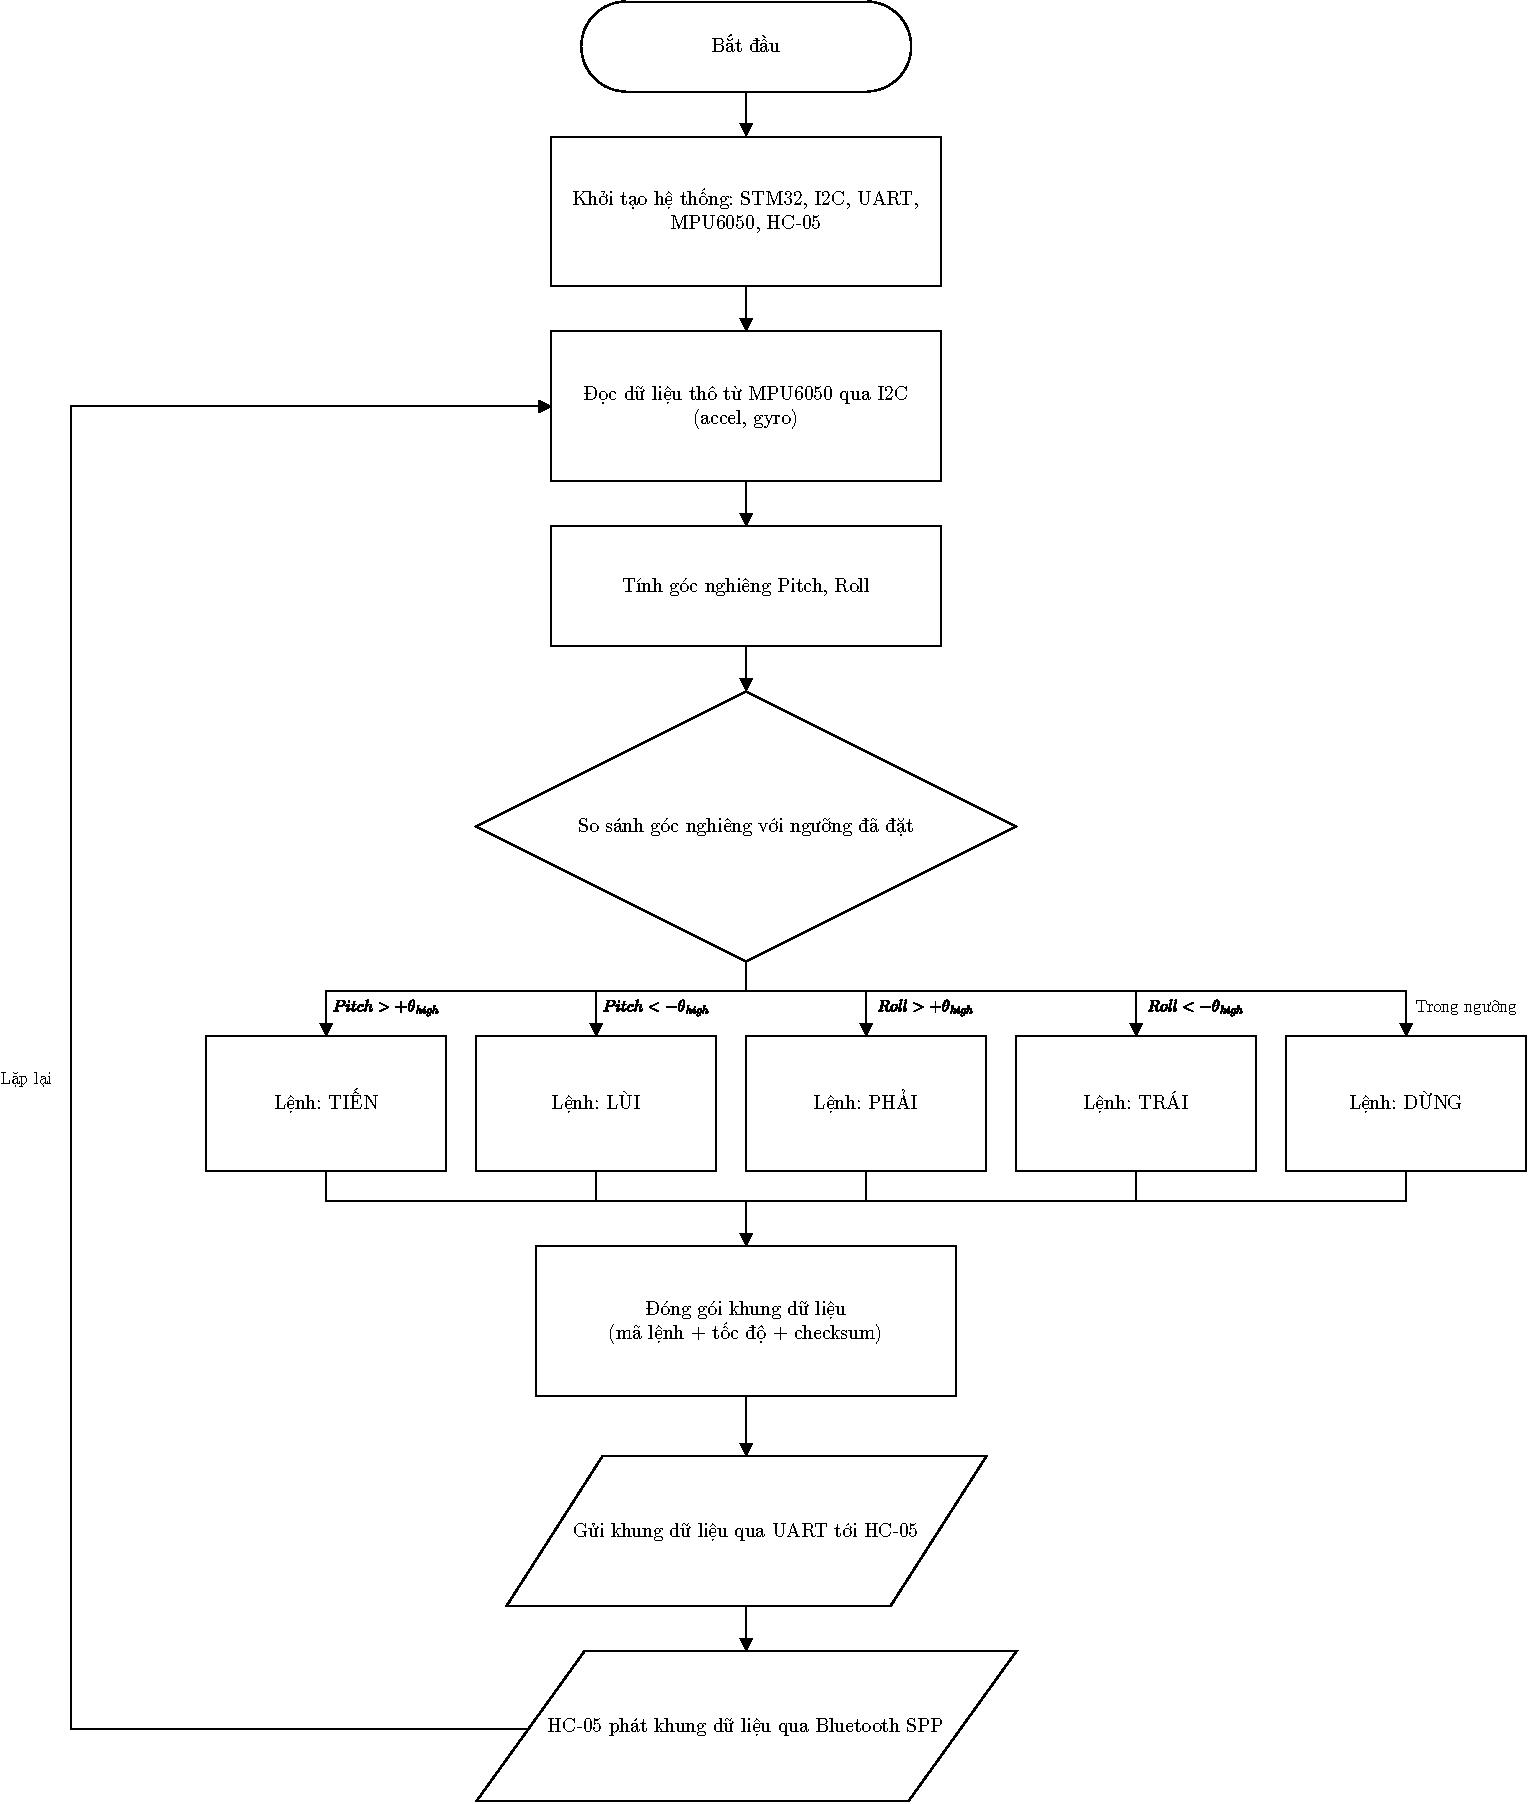
\includegraphics[width=\textwidth, height=0.68\textheight, keepaspectratio]{../Report/Drawio/Transmitter_Flowchart.drawio.pdf}
      \end{center}
    \end{column}
    \begin{column}{0.31\textwidth}
      \begin{block}{Nguyên lý hoạt động}
        \footnotesize
        \begin{itemize}
          \item \textbf{Khởi động:} Cấu hình hệ thống, thiết lập giao tiếp I2C1 và USART1.
          \item \textbf{Calibration:} Thu thập \num{200} mẫu để hiệu chuẩn cảm biến lúc đứng yên.
          \item \textbf{Vòng lặp \qty{10}{\ms}:} 
            \begin{itemize}
              \item Đọc dữ liệu MPU6050.
              \item Lọc Kalman ước lượng góc Pitch/Roll.
              \item Kiểm tra Deadzone và ánh xạ tốc độ phi tuyến.
              \item Đóng gói và gửi chuỗi ký tự qua UART.
            \end{itemize}
        \end{itemize}
      \end{block}
    \end{column}
  \end{columns}
\end{frame}

\begin{frame}{3. Triển khai — Sơ đồ FSM Khối phát}
  \begin{columns}[T]
    \begin{column}{0.65\textwidth}
      \begin{center}
        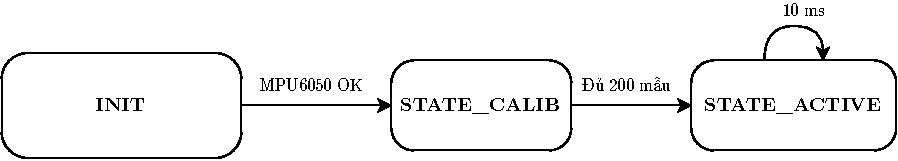
\includegraphics[width=\textwidth, height=0.68\textheight, keepaspectratio]{../Report/Drawio/Transmitter_FSM.drawio.pdf}
      \end{center}
    \end{column}
    \begin{column}{0.31\textwidth}
      \begin{block}{Các trạng thái hoạt động}
        \small
        \begin{itemize}
          \item \texttt{\scriptsize INIT:} Trạng thái khởi tạo phần cứng (MPU6050, Bluetooth, GPIO).
          \item \texttt{\scriptsize IDLE (vùng chết):} Góc nghiêng tay trong dải \qty{\pm 8}{\degree} (Deadzone), gửi lệnh dừng xe.
          \item \texttt{\scriptsize FORWARD / BACKWARD:} Tay nghiêng quá ngưỡng dọc (\qty{\pm 8}{\degree}), gửi lệnh tiến/lùi.
          \item \texttt{\scriptsize LEFT / RIGHT:} Tay nghiêng quá ngưỡng ngang (\qty{\pm 8}{\degree}), gửi lệnh rẽ trái/phải.
        \end{itemize}
      \end{block}
    \end{column}
  \end{columns}
\end{frame}

\begin{frame}{3. Triển khai — Lưu đồ giải thuật Khối thu}
  \begin{columns}[T]
    \begin{column}{0.65\textwidth}
      \begin{center}
        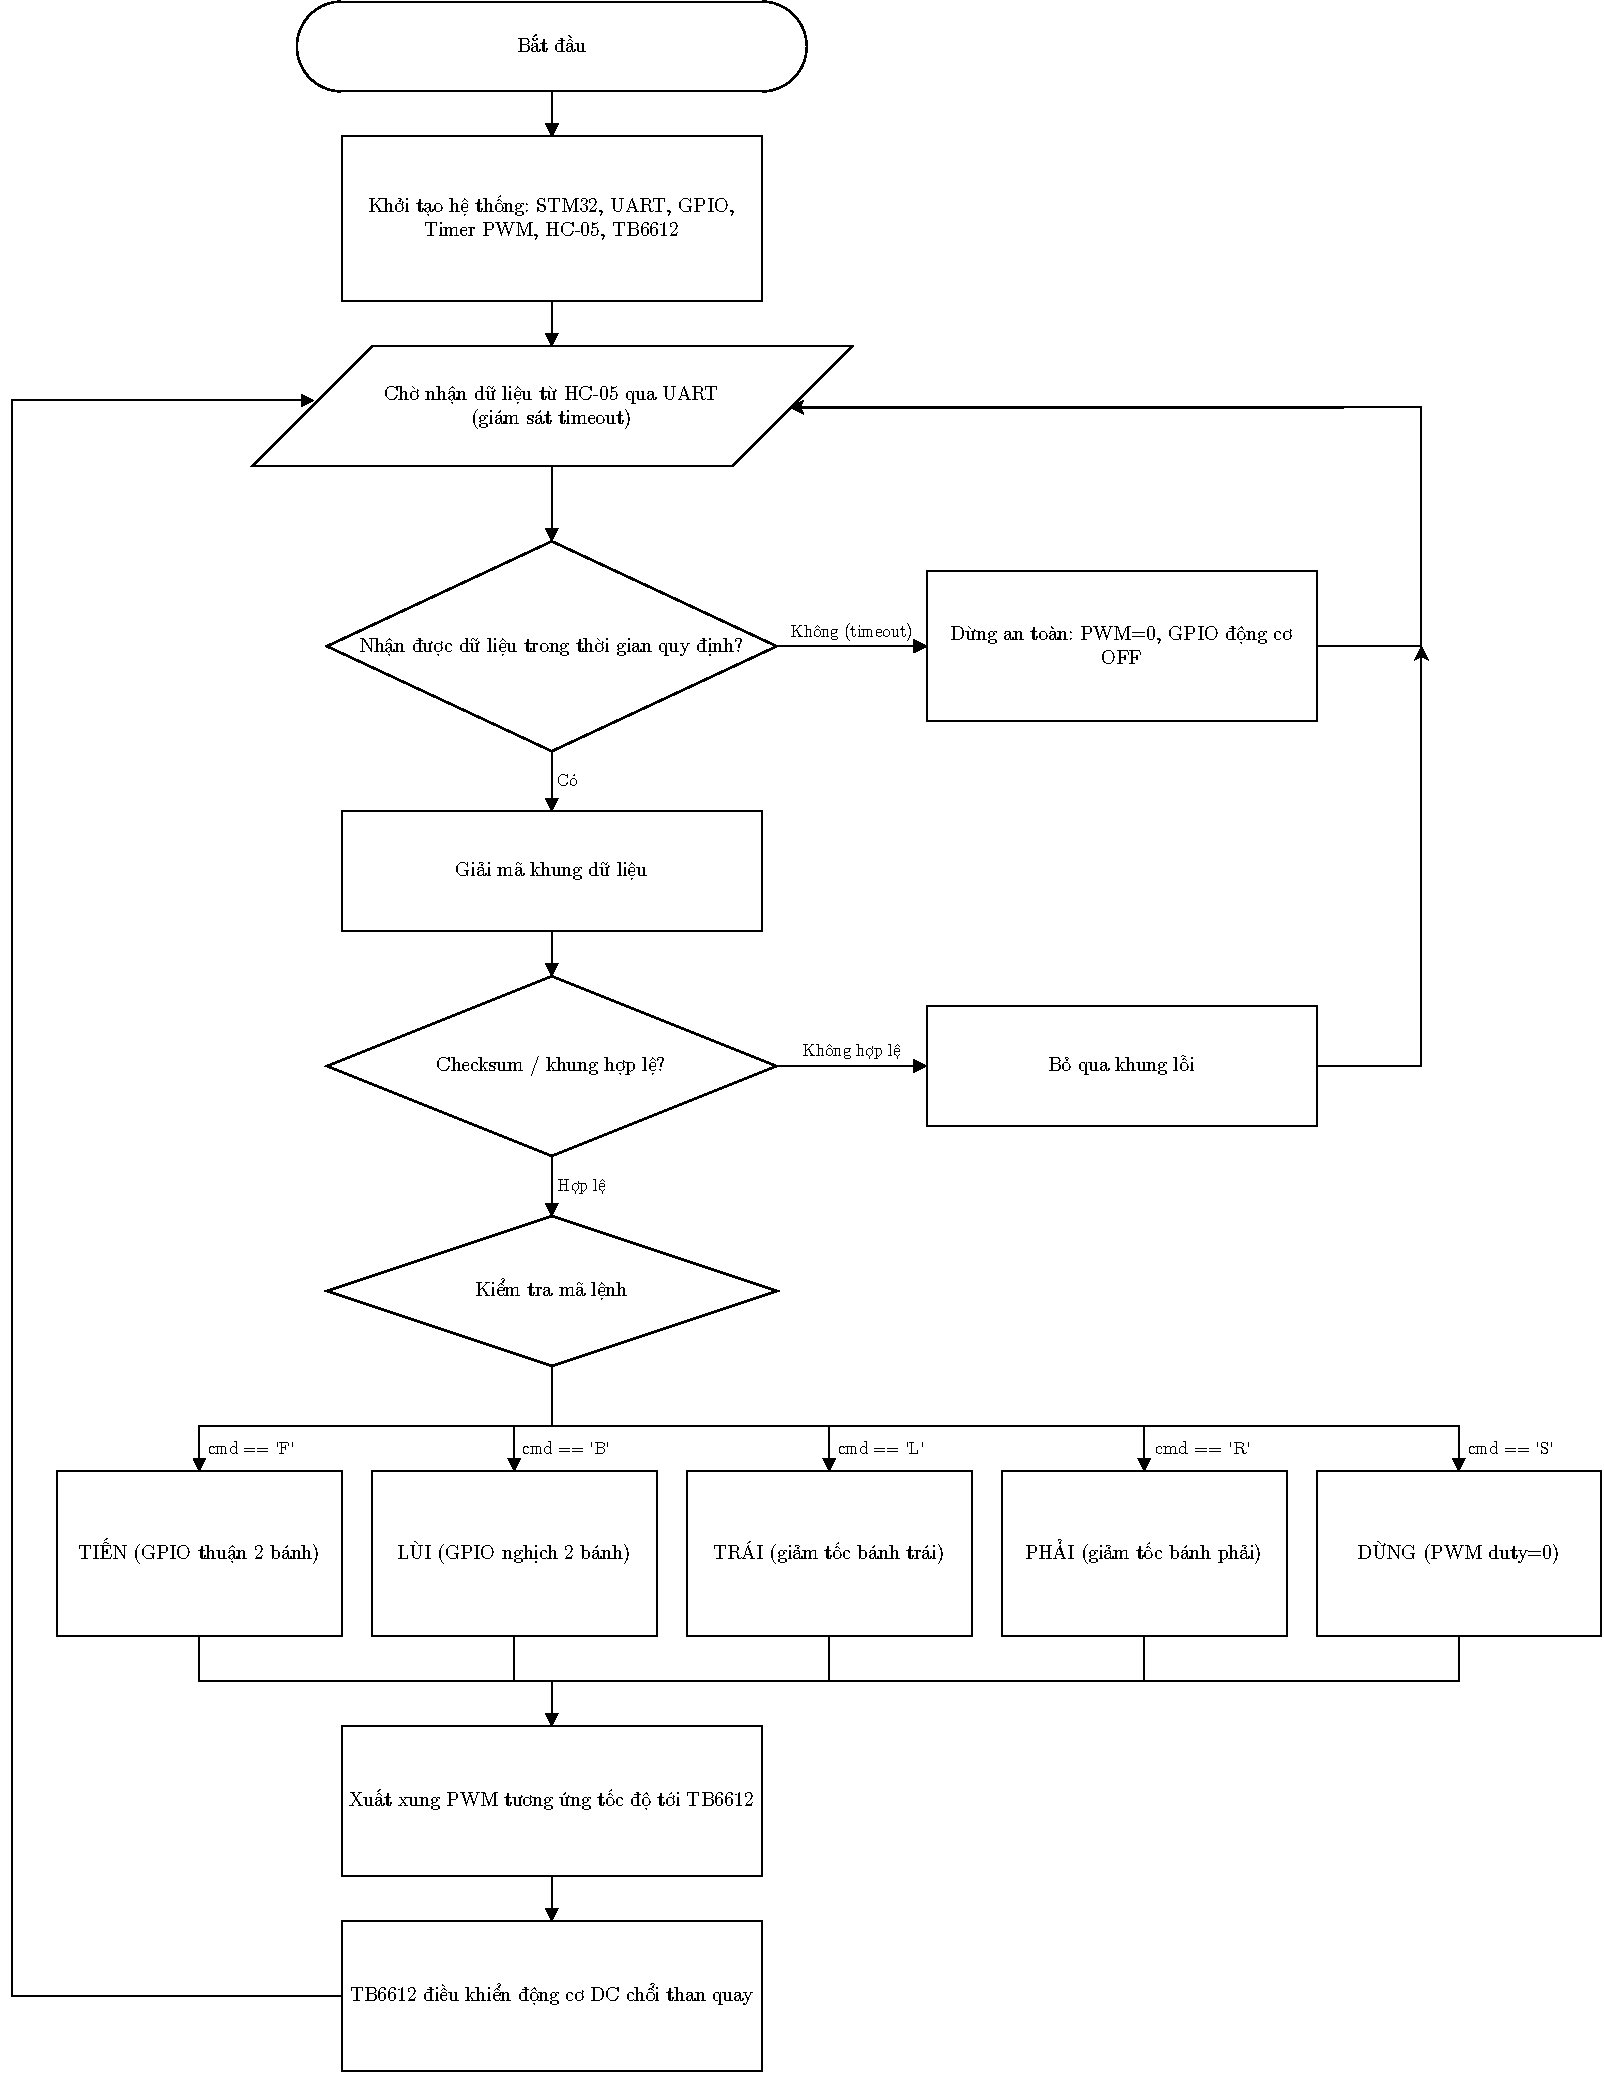
\includegraphics[width=\textwidth, height=0.68\textheight, keepaspectratio]{../Report/Drawio/Receiver_Flowchart.drawio.pdf}
      \end{center}
    \end{column}
    \begin{column}{0.31\textwidth}
      \begin{block}{Nguyên lý hoạt động}
        \footnotesize
        \begin{itemize}
          \item \textbf{Khởi động:} Cấu hình ngắt UART USART1 và cấu hình PWM \qty{10}{\kilo\hertz} trên Timer 2.
          \item \textbf{Vòng lặp chính:}
            \begin{itemize}
              \item Giải mã chuỗi điều khiển `"F:\%d T:\%d"`.
              \item Kiểm tra và kích hoạt cơ chế Fail-safe nếu mất gói tin.
              \item Tính toán điều tốc vi sai bánh xe trái và phải.
              \item Cập nhật hướng GPIO và chu kỳ nhiệm vụ PWM.
            \end{itemize}
        \end{itemize}
      \end{block}
    \end{column}
  \end{columns}
\end{frame}

\begin{frame}{3. Triển khai — Sơ đồ FSM Khối thu}
  \begin{columns}[T]
    \begin{column}{0.65\textwidth}
      \begin{center}
        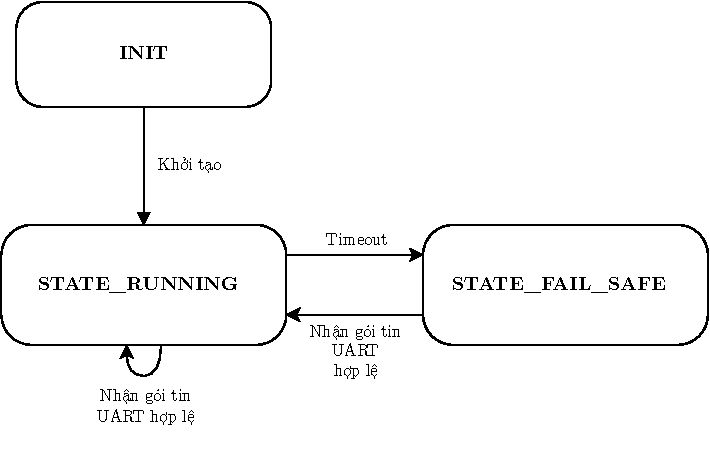
\includegraphics[width=\textwidth, height=0.68\textheight, keepaspectratio]{../Report/Drawio/Receiver_FSM.drawio.pdf}
      \end{center}
    \end{column}
    \begin{column}{0.31\textwidth}
      \begin{block}{Các trạng thái hoạt động}
        \small
        \begin{itemize}
          \item \texttt{\scriptsize INIT \& WAIT\_CONN:} Khởi tạo hệ thống và chờ kết nối Bluetooth.
          \item \texttt{\scriptsize IDLE:} Xe ở trạng thái chờ lệnh di chuyển (dừng động cơ).
          \item \texttt{\scriptsize Điều khiển động cơ:} Các trạng thái di chuyển: \texttt{\scriptsize FORWARD}, \texttt{\scriptsize BACKWARD}, \texttt{\scriptsize TURN\_LEFT}, \texttt{\scriptsize TURN\_RIGHT}.
          \item \texttt{\scriptsize SAFE\_STOP (Fail-safe):} Dừng khẩn cấp khi mất kết nối Bluetooth quá \textbf{\qty{300}{\ms}}.
        \end{itemize}
      \end{block}
    \end{column}
  \end{columns}
\end{frame}

% ------------------------------------------------------------
%  SECTION 4: THỬ NGHIỆM & KẾT QUẢ
% ------------------------------------------------------------
\begin{frame}{4. Thử nghiệm — Kịch bản vận hành thực tế}
  \begin{block}{Thiết lập hệ thống kiểm thử}
    \begin{itemize}
      \item Thiết bị cầm tay: STM32F103 + MPU6050 + Bluetooth Master + Pin Li-ion \qty{3.7}{\volt}.
      \item Xe thử nghiệm: Khung xe 4 bánh DC + STM32F103 + Bluetooth Slave + 2x TB6612 + Pin \qty{7.4}{\volt}.
      \item Địa hình: Mặt phẳng bằng, không vật cản lớn.
    \end{itemize}
  \end{block}
  \begin{block}{Kịch bản điều khiển thực tế}
    \begin{itemize}
      \item \textbf{Tiến / Lùi:} Nghiêng tay cầm trước/sau vượt ngưỡng \qty{\pm 8}{\degree} (xe tiến/lùi với tốc độ tăng dần).
      \item \textbf{Rẽ trái / rẽ phải:} Nghiêng tay cầm sang trái/phải (xe thực hiện rẽ tương ứng nhờ chênh lệch tốc độ).
      \item \textbf{Dừng xe:} Giữ tay cầm thăng bằng trong dải chết \qty{\pm 8}{\degree} (xe phanh dừng hoạt động).
      \item \textbf{Fail-safe:} Ngắt nguồn bộ phát đột ngột (xe lập tức dừng sau \textbf{\qty{300}{\ms}}).
    \end{itemize}
  \end{block}
\end{frame}

\begin{frame}{4. Thử nghiệm — So sánh kết quả các bộ lọc}
  \begin{columns}[T]
    \begin{column}{0.48\textwidth}
      \begin{block}{Đánh giá ưu nhược điểm thực tế}
        \begin{itemize}
          \item \textbf{Chỉ dùng Accelerometer:} Góc phản hồi bị răng cưa rất mạnh do ảnh hưởng của lực rung cơ học khi động cơ hoạt động $\to$ không thể điều khiển mượt.
          \item \textbf{Chỉ dùng Gyroscope:} Góc rất mượt nhưng sai số trôi liên tục tích lũy $\to$ xe tự động trôi/tiến lùi dù tay cầm đứng yên.
          \item \textbf{Dung hợp Kalman Filter:} Tín hiệu góc cực kỳ mượt mà, phản hồi tức thời theo góc nghiêng thực tế của tay cầm và hoàn toàn không bị trôi góc theo thời gian.
        \end{itemize}
      \end{block}
    \end{column}
    \begin{column}{0.48\textwidth}
      \begin{block}{Bảng so sánh chi tiết}
        \centering
        \scriptsize
        \renewcommand{\arraystretch}{1.2}
        \begin{tabular}{|l|c|c|c|}
          \hline
          \textbf{Tiêu chí} & \textbf{Acc} & \textbf{Gyro} & \textbf{Kalman} \\ \hline
          Ổn định tĩnh & Tốt & Kém & Cực tốt \\ \hline
          Đáp ứng động & Chậm & Nhanh & Mượt \\ \hline
          Lọc nhiễu & Kém & Tốt & Rất tốt \\ \hline
          Trôi góc & Không & Có & Không \\ \hline
        \end{tabular}
      \end{block}
    \end{column}
  \end{columns}
\end{frame}

% ------------------------------------------------------------
%  SECTION 5: DEMO THỰC TẾ & ĐÁNH GIÁ
% ------------------------------------------------------------
\begin{frame}{5. Đánh giá — Ưu điểm \& Hạn chế của hệ thống}
  \begin{columns}[T]
    \begin{column}{0.48\textwidth}
      \begin{block}{\textcolor{MLIOTwhite}{Ưu điểm nổi bật}}
        \begin{itemize}
          \item Giao diện điều khiển không dây bằng chuyển động nghiêng trực quan, hiện đại, mang lại trải nghiệm tốt cho người dùng.
          \item Dung hợp cảm biến bằng Kalman Filter đạt hiệu quả cao, tín hiệu lái ổn định và đáp ứng tức thời.
          \item Tần số băm xung điều tốc động cơ \textbf{\qty{10}{\kilo\hertz}} giúp động cơ chạy cực kỳ êm.
          \item Thời gian phản hồi ngắt kết nối an toàn (Fail-safe) phản ứng nhanh (\textbf{\qty{300}{\ms}}).
        \end{itemize}
      \end{block}
    \end{column}
    
    \begin{column}{0.48\textwidth}
      \begin{block}{\textcolor{MLIOTwhite}{Hạn chế hiện tại}}
        \begin{itemize}
          \item Kết nối Bluetooth HC-05 (chuẩn Classic SPP) có phạm vi hoạt động ngắn và dễ bị nhiễu do môi trường xung quanh.
          \item Chỉ chạy tốt trên địa hình bằng phẳng, góc nghiêng lớn dễ gây trượt bánh xe.
          \item Chưa tích hợp cảm biến đo cự ly (như siêu âm) để phanh tự động khi gặp vật cản.
        \end{itemize}
      \end{block}
    \end{column}
  \end{columns}
\end{frame}

% ------------------------------------------------------------
%  SECTION 6: KẾT LUẬN \& HƯỚNG PHÁT TRIỂN
% ------------------------------------------------------------
\begin{frame}{6. Kết luận \& Hướng phát triển}
  \begin{block}{Kết luận chung}
    \begin{itemize}
      \item Đề tài đã hoàn thành việc nghiên cứu, thiết kế phần cứng và lập trình chế tạo thành công prototype xe robot điều khiển bằng góc nghiêng bàn tay.
      \item Thuật toán điều khiển lái vi sai phi tuyến hoạt động chính xác, bộ lọc Kalman ước lượng góc tin cậy, hệ thống phản hồi thời gian thực và an toàn (Fail-safe).
    \end{itemize}
  \end{block}
  \begin{block}{Hướng phát triển tương lai}
    \begin{itemize}
      \item Nâng cấp truyền thông không dây sang chuẩn \textbf{BLE (Bluetooth Low Energy)} hoặc kết nối mạng \textbf{Wi-Fi} để tăng tầm xa và độ ổn định.
      \item Tích hợp cảm biến quán tính IMU cao cấp hơn (như BNO055 tích hợp sẵn bộ vi xử lý hướng góc) để giảm tải cho STM32.
      \item Tích hợp các cảm biến siêu âm, LiDAR để bổ sung tính năng phanh tránh vật cản tự động.
    \end{itemize}
  \end{block}
\end{frame}

% ------------------------------------------------------------
%  SLIDE 16 – Thank You / Acknowledgements
% ------------------------------------------------------------
\thankyouslide{%
  Nhóm thực hiện chân thành cảm ơn anh Võ Quang Vinh cùng các anh hướng dẫn tại Machine Learning \& IoT Lab đã tận tình hướng dẫn, hỗ trợ kỹ thuật và tạo điều kiện thuận lợi nhất để nhóm hoàn thành đề tài nghiên cứu này.
}

% ============================================================
\end{document}
% ============================================================
